% Created 2024-04-08 Mon 21:06
% Intended LaTeX compiler: pdflatex
\documentclass[a4paper, 11pt]{article}
\usepackage[utf8]{inputenc}
\usepackage[T1]{fontenc}
\usepackage{graphicx}
\usepackage{longtable}
\usepackage{wrapfig}
\usepackage{rotating}
\usepackage[normalem]{ulem}
\usepackage{amsmath}
\usepackage{amssymb}
\usepackage{capt-of}
\usepackage{hyperref}
\usepackage{lmodern} % Ensures we have the right font
\usepackage[T1]{fontenc}
\usepackage{inputenc}
\usepackage{graphicx, float}
\usepackage{amsmath, amsfonts, amsthm, amssymb, lipsum}
\usepackage[table, xcdraw]{xcolor}
\usepackage[colorlinks]{hyperref}
\hypersetup{colorlinks, linkcolor=blue, urlcolor=blue}
\setlength{\parindent}{0pt}
\setlength{\parskip}{1em}
\usepackage[stretch=10]{microtype}
\usepackage{hyphenat}
\usepackage{ragged2e}
\usepackage{subfig} % Subfigures (not needed in Org I think)
\usepackage{hyperref} % Links
\usepackage{listings} % Code highlighting
\usepackage[margin=1in, footskip=0.25in]{geometry}
\renewcommand{\baselinestretch}{1.15}
\pagenumbering{gobble}
\usepackage[explicit]{titlesec}
\usepackage{enumitem}
\setlist[itemize]{topsep=0pt}
\newtheorem{theorem}{Theorem}[section]
\newtheorem{corollary}{Corollary}[theorem]
\newtheorem{lemma}[theorem]{Lemma}
\newtheorem{definition}{Definition}[theorem]
\setlength{\abovedisplayskip}{-15pt}
\setlength{\belowdisplayskip}{0pt}
\setlength{\abovedisplayshortskip}{0pt}
\setlength{\belowdisplayshortskip}{0pt}
\author{Bryan Lim Jing Xiang (A0233605M)}
\date{}
\title{Task B1}
\hypersetup{
 pdfauthor={Bryan Lim Jing Xiang (A0233605M)},
 pdftitle={Task B1},
 pdfkeywords={},
 pdfsubject={},
 pdfcreator={Emacs 29.3 (Org mode 9.7)}, 
 pdflang={English}}
\begin{document}

\maketitle
\section{Dataset}
\label{sec:org2dcf744}
\subsection{Overview}
\label{sec:org2f62eb1}
This dataset consists of the population breakdown of Singapore from 2000 to 2020. The data fields that are of interest here are:

\begin{center}
\begin{tabular}{lll}
Field & Description & Data Type\\[0pt]
\hline
Year & Year & Integer\\[0pt]
Group & Denoting the residents that are included in the group & String\\[0pt]
Age Group & Age group & String\\[0pt]
Value & Number of residents belonging to the particular group & Integer\\[0pt]
\end{tabular}
\end{center}

This dataset is interesting in that it allows us to analyse the popularity and trends in the anime industry across many different years and seasons.
\subsection{Data origin}
\label{sec:orga4296b2}
\url{https://docs.google.com/spreadsheets/d/1a2uZKydzbP-vTdrXrdcGmfxTFnZSXdDS65XOpjWY0SE/edit\#gid=1367742117}
\subsection{Github Repository}
\label{sec:org9233c79}
\url{https://github.com/bryanljx/visualisation}
\section{Purpose of Visualisation}
\label{sec:org4df4e70}
For this dataset, the query of interest is: ``How fast is Singapore's population ageing? Is ageing population really a huge issue?''
\section{Visualisation}
\label{sec:org07249ab}
\subsection{Comparison of Population Pyramid across 2000, 2010, and 2020}
\label{sec:org184417f}

\begin{center}
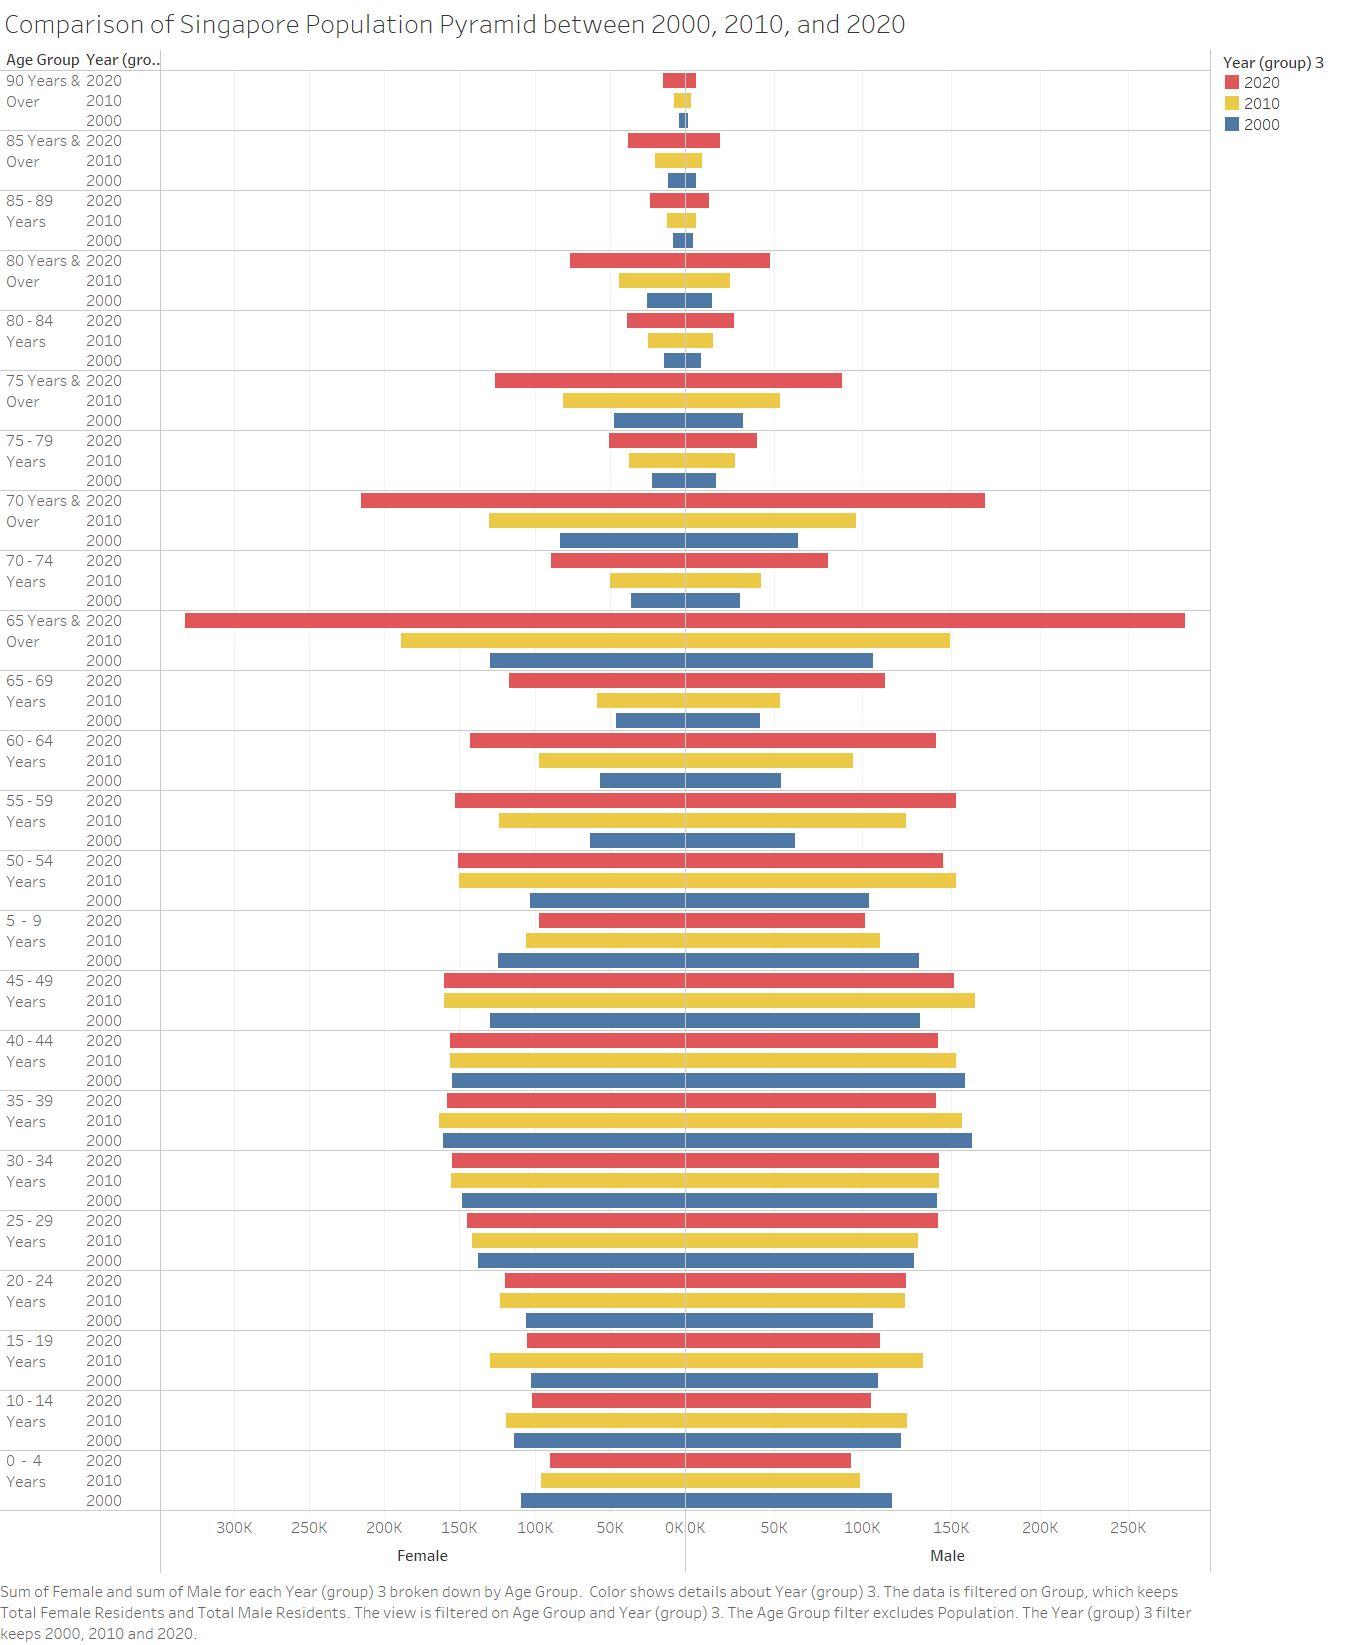
\includegraphics[width=.9\linewidth]{./charts/Pyramid.png}
\end{center}

\begin{itemize}
\item Visual encoding here includes:
\begin{itemize}
\item Length - Denoting the amount of residents (male/female) for each age group
\item Color - Differentiating the year - 2000/2010/2020
\item Position - Denoting the age group
\end{itemize}
\item Insights
\begin{itemize}
\item Clearly, the number of elderly are increasing rather substantially across the decades whereas the converse is not true for young adults
\end{itemize}
\end{itemize}
\subsection{Old Age Support Ratio}
\label{sec:org98c4f7d}

\begin{center}
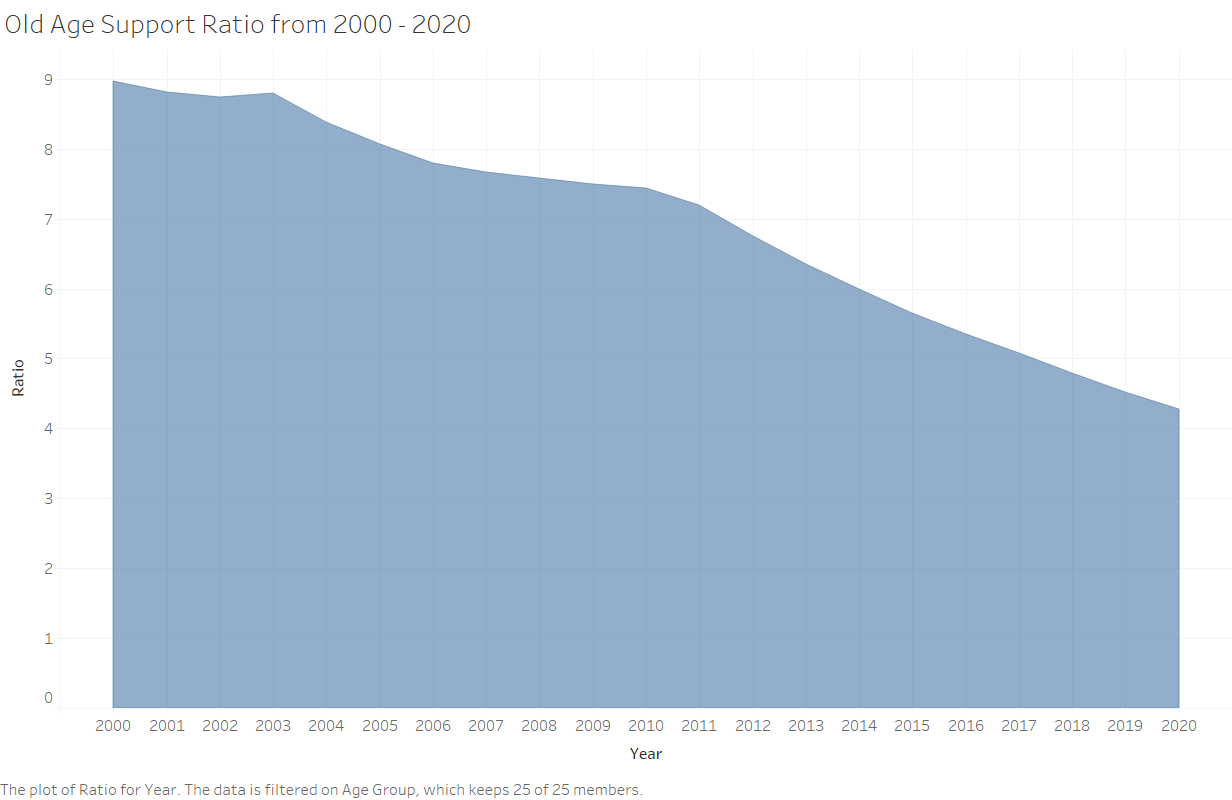
\includegraphics[width=.9\linewidth]{./charts/old age support ratio.png}
\end{center}

\begin{itemize}
\item As the name implies, old age support ratio is the ratio of working adults to elderly
\item An area chart was chosen to emphasise the decreasing pattern across time.
\item Visual encoding here includes:
\begin{itemize}
\item Position - Denoting the ratio
\end{itemize}
\item Insights
\begin{itemize}
\item From the chart, it is evident how this is decreasing over time at a very steady pace
\end{itemize}
\end{itemize}
\subsection{Percentage of elderly amongst the population across time}
\label{sec:orgc4363db}

\begin{center}
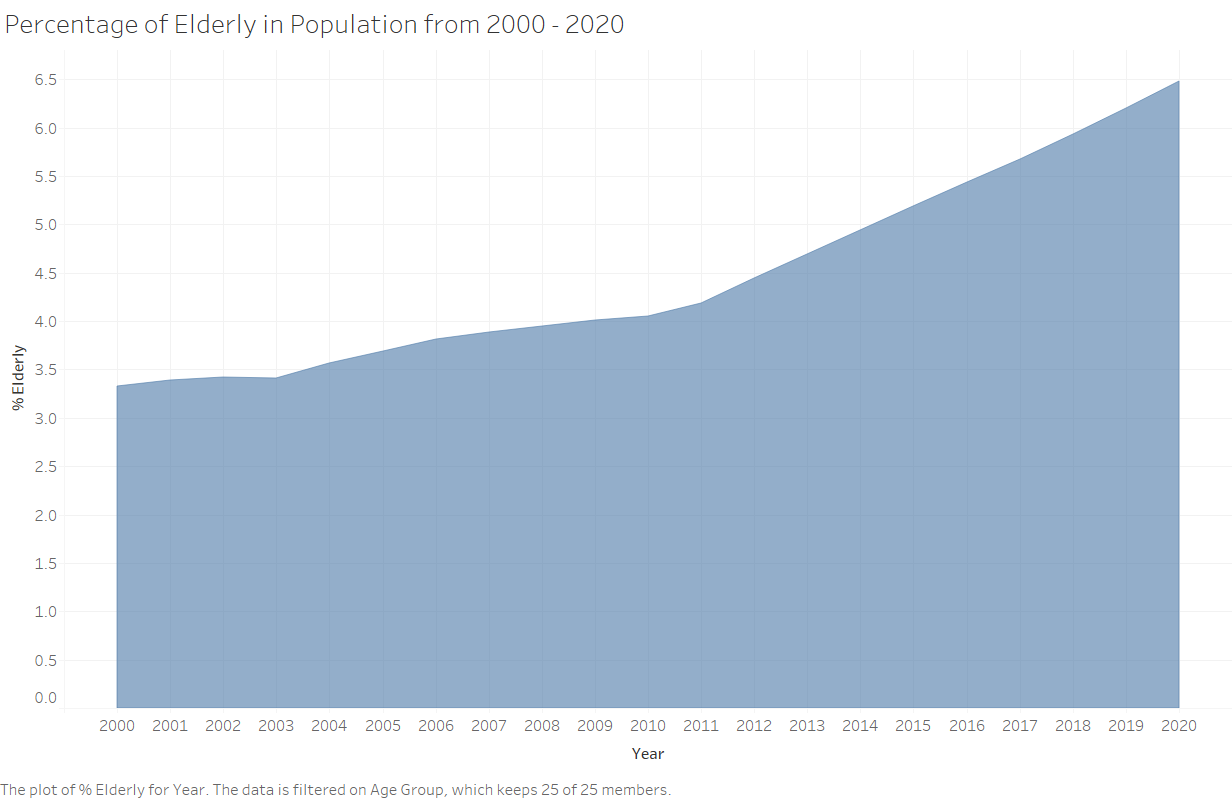
\includegraphics[width=.9\linewidth]{./charts/% elderly.png}
\end{center}

\begin{itemize}
\item An area chart was chosen to emphasise the increasing percentage across time.
\item Visual encoding here includes:
\begin{itemize}
\item Position - Denoting the percentage of elderly amongst the population
\end{itemize}
\item Insights
\begin{itemize}
\item The rate of increase seems to be picking up in recent years which is concerning
\end{itemize}
\end{itemize}
\end{document}
